\documentclass[conference]{IEEEtran}

\usepackage[T1]{fontenc}
\usepackage[utf8]{inputenc}
\usepackage{graphicx}
\usepackage{amsmath}
\usepackage{booktabs}
\usepackage{array}
\usepackage{tabularx}
\usepackage{cite}
\usepackage{url}
\usepackage{microtype}
\usepackage{balance}

\newcolumntype{Y}{>{\raggedright\arraybackslash}X}
\newcolumntype{L}[1]{>{\raggedright\arraybackslash}p{#1}}


\title{Self-Auditing Clinical Decision Support Agent: An Agentic AI Architecture for Trustworthy Clinical Decision Support}

\author{\IEEEauthorblockN{Bhargav Boyapati}
\IEEEauthorblockA{University of Texas at Arlington\\
Arlington, Texas, USA\\
Email: bhargavboyapati2602@gmail.com}}

\begin{document}
\maketitle
\begin{abstract}
Clinical decision support systems increasingly use machine learning and large language models to generate risk scores, explanations, and recommendations. However, prediction quality alone is not enough for trustworthy clinical AI. Clinical users need outputs that are evidence-grounded, traceable, reviewable, and safe to withhold when evidence is weak. This paper presents a literature-informed architecture for a Self-Auditing Clinical Decision Support Agent. The proposed system combines interpretable risk prediction, clinical evidence retrieval, evidence-constrained reasoning, claim-level self-auditing verification, and reliability scoring. The core design principle is simple: no evidence, no claim. The system is positioned as a research prototype using simulated patient cases and guideline-style evidence, not as a clinically validated diagnostic engine. The contribution is an end-to-end agentic architecture that separates prediction, retrieval, reasoning, verification, and output generation into auditable layers.
\end{abstract}

\begin{IEEEkeywords}
Agentic AI, clinical decision support, trustworthy AI, retrieval-augmented generation, self-auditing AI, explainable AI, healthcare AI, reliability scoring.
\end{IEEEkeywords}

\section{Introduction}
Clinical decision support systems (CDSS) have long aimed to assist clinicians with evidence-based recommendations at the point of care. With the rapid adoption of machine learning (ML) and large language models (LLMs), these systems can now generate risk scores, summaries, and free-text recommendations. Yet a persistent trust gap remains: many systems produce outputs without clearly showing how those outputs were generated, whether they are supported by clinical evidence, or when they should not be trusted.

This paper reformats and condenses a literature survey into an IEEE-style research paper centered on a Self-Auditing Clinical Decision Support Agent. The proposed architecture moves from a prediction-only pipeline,
\begin{center}
\textit{Input $\rightarrow$ Model $\rightarrow$ Output},
\end{center}
into a verifiable pipeline,
\begin{center}
\textit{Input $\rightarrow$ Prediction $\rightarrow$ Evidence $\rightarrow$ Reasoning $\rightarrow$ Verification $\rightarrow$ Output}.
\end{center}
The goal is not to replace clinician judgment. Instead, the system is designed to make AI-assisted clinical reasoning more transparent by exposing evidence alignment, unsupported claims, and reliability signals before recommendations are presented.

\section{Research Motivation}
Prediction alone is insufficient for trustworthy clinical AI. A model may output an accurate risk score, but clinical users still need to understand why the output was generated, how it relates to patient-specific evidence, and whether the recommendation exceeds the supporting evidence. Trust is therefore not a byproduct of accuracy. It is a system-level property requiring transparency, usability, clinical reliability, validation, ethical design, and clinician control.

The literature survey behind this work is guided by six research questions listed in Table~\ref{tab:research_questions}. These questions shape the proposed architecture and evaluation plan.

\begin{table}[t]
\caption{Research Questions Guiding the Work}
\label{tab:research_questions}
\centering
\scriptsize
\begin{tabularx}{\linewidth}{L{0.15\linewidth}Y}
\toprule
\textbf{ID} & \textbf{Research Question} \\
\midrule
RQ1 & Why is prediction alone insufficient for trustworthy clinical AI? \\
RQ2 & What methods exist for grounding clinical AI in evidence? \\
RQ3 & How do current systems verify or audit their own reasoning? \\
RQ4 & What architectural patterns support transparent, modular clinical AI? \\
RQ5 & What evaluation frameworks exist for trustworthiness beyond accuracy? \\
RQ6 & Where are the gaps that a self-auditing CDS architecture can address? \\
\bottomrule
\end{tabularx}
\end{table}

\section{Background and Related Work}
\subsection{Clinical Decision Support and the Trust Gap}
Early CDSS research emphasized rule-based expert systems and computable clinical practice guidelines. These systems were interpretable, but often difficult to scale and maintain. Modern ML-based CDSS improved predictive performance across domains such as cardiovascular risk, sepsis, and diagnostic imaging, but interpretability concerns intensified as models became more complex. Prior work has noted that clinical prediction models often face a tradeoff between accuracy and interpretability \cite{lacava2023}.

Trust in AI-based CDSS is multidimensional. Healthcare workers need transparent system behavior, usability, clinical reliability, credibility, validation across diverse contexts, fairness, accountability, and preservation of clinician autonomy \cite{trust2025}. This motivates architectures that expose not only the final recommendation, but also the evidence and audit trace behind it.

\subsection{Interpretable Risk Prediction}
Logistic regression remains a strong baseline for clinical risk prediction because it is fast, probabilistic, and interpretable. Coefficients can be inspected, feature contributions can be communicated, and outputs can be calibrated for tabular clinical data \cite{hosmer2013}. More complex approaches such as Explainable Boosting Machines, XGBoost with SHAP, and deep learning can improve task-level performance, but post-hoc explanations do not guarantee that downstream recommendations are clinically faithful or evidence-grounded.

For a research-grade prototype, interpretable prediction provides an appropriate first layer. The key design choice is to treat risk prediction as one component in a larger reasoning system, not as the final clinical output.

\subsection{Evidence Retrieval and RAG in Healthcare}
Clinical information retrieval supports access to relevant evidence from clinical practice guidelines, literature, and EHR-style corpora. TF-IDF and BM25 remain useful retrieval baselines because they are lightweight and inspectable \cite{sparckjones1972}. Retrieval-augmented generation (RAG) extends this idea by grounding LLM outputs in retrieved context. Recent healthcare RAG studies show improved performance compared with baseline LLMs, especially when retrieval is paired with stronger system-level design \cite{ragmeta2025,ragreview2025}.

However, retrieval alone does not guarantee faithful reasoning. A system can retrieve relevant evidence and still generate claims that go beyond, misinterpret, or contradict that evidence. This limitation motivates a dedicated verification layer.

\subsection{Self-Verification and Claim-Level Auditing}
Self-verification refers to systems that check their own outputs before presentation. In clinical information extraction, self-verification pipelines have improved accuracy by detecting omissions, grounding extracted elements, and pruning unsupported outputs \cite{selfverification2023}. Biomedical RAG verification has also moved toward atomic claim decomposition, natural language inference, and evidence-quality scoring \cite{medragchecker2026,verirag2025}.

The central insight is that generation and verification are asymmetric. It may be easier for a model or rule-based verifier to check whether a claim is supported than to generate a fully correct clinical answer in one pass. The proposed architecture uses this asymmetry by auditing claims before final output.

Table~\ref{tab:prior_comparison} summarizes how the proposed architecture differs from closely related system families. The main distinction is that this work connects prediction, retrieval, reasoning, and verification into one auditable clinical decision-support pipeline.

\begin{table*}[t]
\caption{Comparison with Prior Work and Related System Patterns}
\label{tab:prior_comparison}
\centering
\scriptsize
\begin{tabularx}{\textwidth}{L{0.18\textwidth} L{0.23\textwidth} L{0.24\textwidth} Y}
\toprule
\textbf{Prior Work} & \textbf{Focus} & \textbf{Limitation} & \textbf{This Work's Contribution} \\
\midrule
Traditional CDSS & Risk prediction and rule-based alerts & Limited reasoning trace and weak connection between prediction and supporting evidence & Adds evidence retrieval, audit trace, and reliability scoring to decision-support output \\
Basic RAG & Retrieval-grounded answers using external documents & Retrieves evidence but does not verify every generated claim & Adds a self-auditing layer that checks claim support before presentation \\
Self-RAG & Retrieve, generate, and critique using self-reflection & General-domain pattern that is not designed specifically for clinical CDS workflows & Applies retrieval and critique principles to evidence-constrained clinical decision support \\
MedRAGChecker & Biomedical claim verification for RAG answers & Primarily focused on biomedical QA rather than full CDS pipelines & Extends claim-level verification toward patient-data-driven CDS output \\
FUTURE-AI & Trustworthy healthcare AI principles and lifecycle guidance & Provides guideline-level principles rather than an implementation architecture & Operationalizes traceability, explainability, and auditability in a prototype system design \\
\bottomrule
\end{tabularx}
\end{table*}

\section{Proposed Architecture}
The Self-Auditing Clinical Decision Support Agent is organized as a modular agentic pipeline. Each layer has a narrow responsibility: patient data input, clinical feature processing, risk prediction, evidence retrieval, evidence-constrained reasoning, self-auditing verification, reliability scoring, and transparent clinical output.

\begin{figure*}[t]
\centering
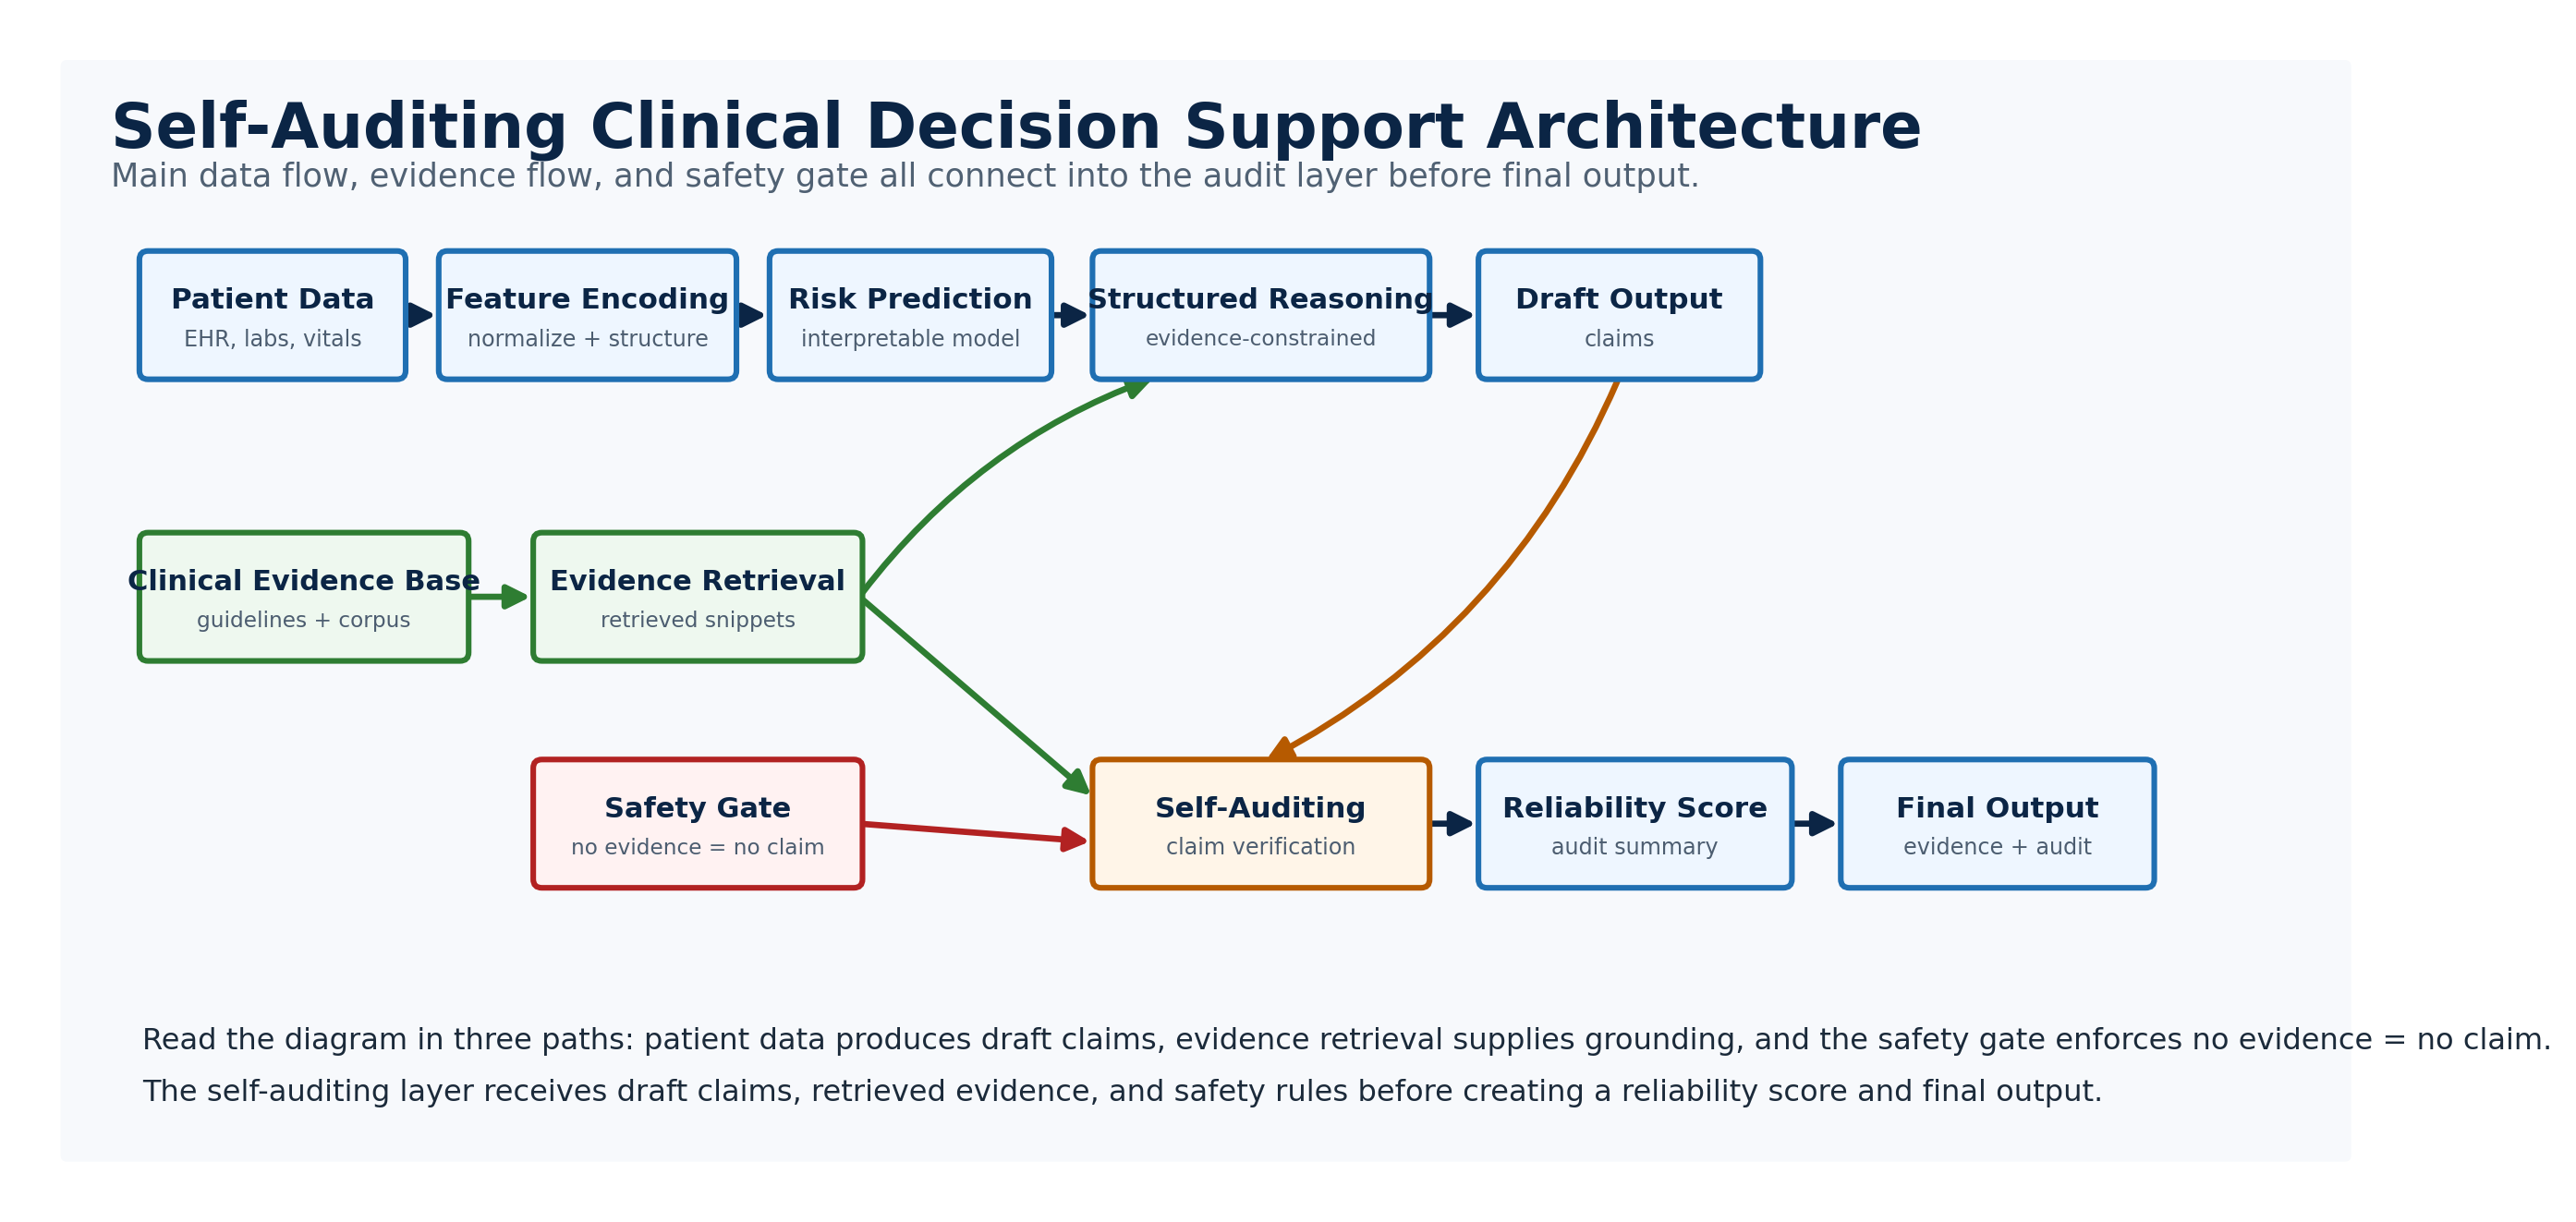
\includegraphics[width=0.96\textwidth]{architecture_clear.png}
\caption{Clear end-to-end Self-Auditing Clinical Decision Support Architecture. Blue components show the patient-data and reasoning path, green components show evidence and reliability layers, orange shows verification, and red shows the no-evidence-no-claim safety gate.}
\label{fig:architecture}
\end{figure*}

The architecture in Fig.~\ref{fig:architecture} separates model prediction from clinical reasoning. This matters because a risk score alone does not provide enough context for decision support. The evidence retrieval layer fetches guideline-style evidence. The structured reasoning layer generates recommendations under evidence constraints. The verification layer then checks whether generated claims are supported, weakly supported, unsupported, or unsafe. Finally, a reliability score summarizes audit quality.

Fig.~\ref{fig:architecture} should be read as three connected paths. First, the data path converts patient case information into structured features and an interpretable risk prediction. Second, the evidence path retrieves guideline-style support from the clinical evidence base and passes it into the reasoning layer. Third, the audit path checks every generated claim before final output. The red safety gate applies the core rule: if the system cannot find enough evidence for a claim, the claim must be flagged, rewritten, or withheld.


\subsection{Risk Prediction Layer}
The risk prediction layer uses interpretable models such as logistic regression in the initial phase. The purpose is not to maximize benchmark performance at all costs. The purpose is to provide a transparent risk signal that can be checked against recommendations. For example, a high-risk classification should align with a higher-urgency recommendation, while a low-risk classification should not trigger unsupported escalation.

\subsection{Evidence Retrieval Layer}
The evidence retrieval layer retrieves clinical guideline-style passages using lightweight methods such as TF-IDF with cosine similarity in Phase 1. BM25, dense embeddings, hybrid retrieval, reranking, and citation-aware retrieval can be introduced in later phases. Table~\ref{tab:retrieval} summarizes the retrieval design choices.

\begin{table}[t]
\caption{Evidence Retrieval Options}
\label{tab:retrieval}
\centering
\scriptsize
\begin{tabularx}{\linewidth}{L{0.30\linewidth}Y L{0.22\linewidth}}
\toprule
\textbf{Method} & \textbf{Strength} & \textbf{Role} \\
\midrule
TF-IDF + cosine similarity & Fast, interpretable, lightweight, and easy to audit for guideline-style retrieval. & Phase 1 baseline \\
BM25 & Improves lexical ranking through probabilistic scoring and document-length normalization. & Phase 2 upgrade \\
Dense embeddings & Better semantic matching and paraphrase handling. & Phase 2 upgrade \\
Hybrid retrieval + reranking & Combines lexical and semantic signals for stronger recall and precision. & Phase 2--3 upgrade \\
\bottomrule
\end{tabularx}
\end{table}

\subsection{Evidence-Constrained Reasoning}
The reasoning layer follows the rule: \textit{no evidence, no claim}. A recommendation should only be generated when supporting evidence is retrieved and aligned with the patient case. Claims that exceed the evidence should be flagged rather than silently presented.

This layer is intentionally structured rather than fully free-form. It decomposes clinical output into interpretable components such as risk signal, retrieved evidence, possible concerns, recommendation summary, and uncertainty notes. This structure makes the output easier to verify.

\subsection{Self-Auditing Verification Layer}
The self-auditing layer performs claim-level verification before final presentation. It extracts atomic claims from the generated recommendation and compares them against the retrieved evidence set. The output can be classified as supported, weakly supported, unsupported, contradictory, or unsafe.

\begin{figure*}[t]
\centering
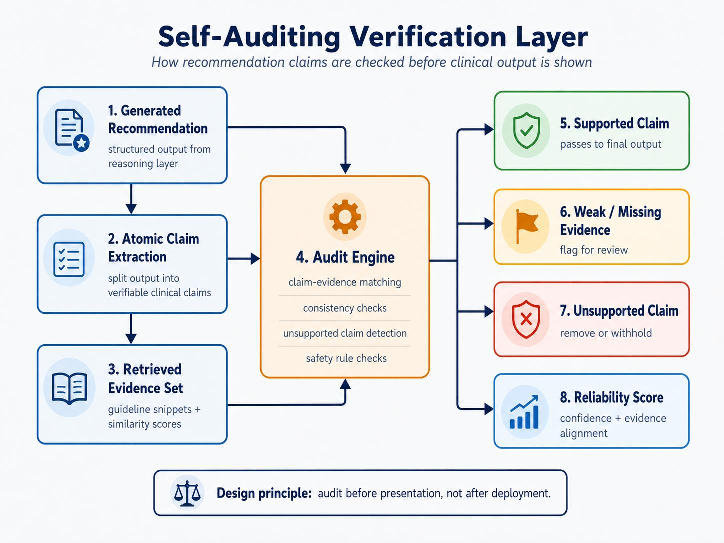
\includegraphics[width=0.92\textwidth]{verification_clear.pdf}
\caption{Clear self-auditing verification layer. Draft recommendations are split into atomic claims, matched against retrieved evidence, and classified as supported, weakly supported, unsupported/contradictory, or converted into a reliability score.}
\label{fig:verification}
\end{figure*}

Fig.~\ref{fig:verification} shows the verification layer as an audit engine that receives generated recommendations, extracted atomic claims, and retrieved evidence. The verifier produces supported claims, weak or missing evidence flags, unsupported claim decisions, and reliability scores.

This layer is the main safety differentiator in the proposed system. A basic RAG system may retrieve useful context and still produce unsupported statements. In contrast, this verifier explicitly compares each atomic claim against the retrieved evidence set before the recommendation reaches the final clinical decision-support output.


\section{Reliability Scoring}
Reliability scoring converts multiple audit signals into a transparent trust indicator. The score should not be interpreted as proof of clinical correctness. Instead, it describes how well the output is grounded in retrieved evidence and whether safety constraints were violated. Table~\ref{tab:reliability} lists key reliability signals.

\begin{table}[t]
\caption{Reliability Scoring Signals}
\label{tab:reliability}
\centering
\scriptsize
\begin{tabularx}{\linewidth}{L{0.38\linewidth}Y}
\toprule
\textbf{Signal} & \textbf{Purpose} \\
\midrule
Claim support rate & Measures the proportion of generated claims supported by retrieved evidence. \\
Evidence relevance & Measures whether retrieved passages match the patient case and recommendation. \\
Unsupported claim rate & Tracks claims that cannot be grounded in retrieved evidence. \\
Contradiction detection & Flags claims that conflict with evidence or clinical constraints. \\
Prediction-recommendation consistency & Checks whether the recommendation aligns with the predicted risk level. \\
Safety rule violations & Detects unsafe or out-of-scope outputs such as unsupported diagnostic claims. \\
Explanation fidelity & Evaluates whether the explanation reflects the model output and evidence. \\
\bottomrule
\end{tabularx}
\end{table}

A practical scoring function can combine support rate, evidence relevance, contradiction penalties, unsupported-claim penalties, and safety-rule penalties. For a prototype, the exact scoring weights should be transparent and manually reviewable.

\section{Research Gaps and Contribution}
The literature identifies six gaps that motivate this work: prediction-reasoning disconnect, retrieval without verification, post-hoc explainability, missing reliability scoring, monolithic architectures, and limited end-to-end CDS evaluation.

This project addresses those gaps through an integrated architecture that:
\begin{itemize}
    \item combines interpretable risk prediction with evidence retrieval;
    \item enforces evidence-constrained reasoning through a no-evidence-no-claim rule;
    \item introduces a dedicated self-auditing verification layer;
    \item produces reliability scores based on audit results;
    \item generates transparent output containing risk, evidence, recommendation, audit trace, and safety disclaimer;
    \item uses modular agentic components that can be independently evaluated and improved.
\end{itemize}

Compared with standard RAG systems, this architecture does not stop at retrieving context. It explicitly verifies whether generated claims are supported by retrieved evidence. Compared with prediction-only CDSS, it connects risk prediction to evidence-grounded reasoning and audit scoring.

\section{Evaluation Plan}
The proposed system should be evaluated using simulated patient cases and guideline-style evidence. The evaluation should focus on whether the system retrieves relevant evidence, keeps generated claims grounded, flags unsupported reasoning, and produces reliability scores that are meaningful under manual review. Table~\ref{tab:evaluation_plan} lists the core prototype metrics.

\begin{table}[!htbp]
\caption{Evaluation Metrics for the Prototype Study}
\label{tab:evaluation_plan}
\centering
\scriptsize
\begin{tabularx}{\linewidth}{L{0.40\linewidth}Y}
\toprule
\textbf{Metric} & \textbf{What It Evaluates} \\
\midrule
Evidence support rate & Percentage of generated claims that are supported by retrieved evidence. \\
Unsupported claim rate & Percentage of claims flagged because the evidence is missing, weak, or insufficient. \\
Retrieval relevance & Whether retrieved guideline-style passages are relevant to the patient case and recommendation. \\
Prediction-recommendation consistency & Whether the generated recommendation logically aligns with the predicted risk level. \\
Reliability score distribution & How reliability scores behave across low-risk, medium-risk, high-risk, and ambiguous cases. \\
Manual review agreement & Agreement between automated audit labels and human review of claim-evidence alignment. \\
\bottomrule
\end{tabularx}
\end{table}


\section{Future Enhancements}
The current prototype is intentionally lightweight so that each decision-support step can be inspected and evaluated. Future work should improve retrieval quality, verification depth, clinician review, and governance readiness without weakening the core auditability of the system. Table~\ref{tab:future_enhancements} summarizes the most important planned enhancements.

\begin{table}[!htbp]
\caption{Planned Future Enhancements}
\label{tab:future_enhancements}
\centering
\scriptsize
\begin{tabularx}{\linewidth}{L{0.37\linewidth}Y}
\toprule
\textbf{Enhancement} & \textbf{Purpose} \\
\midrule
Hybrid retrieval and reranking & Combine BM25, dense embeddings, and reranking to improve evidence recall while keeping retrieved passages traceable. \\
NLI-based claim verification & Extend rule-based auditing with entailment, contradiction, and under-evidence detection at the atomic-claim level. \\
Clinician review interface & Present risk score, retrieved evidence, audit labels, reliability score, and unsupported-claim warnings in a reviewable UI. \\
Simulated benchmark cases & Build annotated patient-case sets with expected evidence links, claim labels, and manual review outcomes. \\
Fairness and subgroup analysis & Evaluate retrieval, prediction, and audit performance across simulated demographic and clinical subgroups. \\
Governance and observability layer & Add audit logs, version tracking, monitoring, drift checks, and PHI-aware controls for translation-ready research. \\
\bottomrule
\end{tabularx}
\end{table}

Additional technical extensions include FHIR-compatible input formatting, citation-aware retrieval, confidence calibration, failure-mode dashboards, and comparison against basic RAG and prediction-only baselines. These enhancements should be introduced after the Phase 1 prototype demonstrates that claim-level auditing can reduce unsupported clinical reasoning on simulated cases.

\section{Safe Positioning}
Safe positioning is essential. This system is a research prototype, not a diagnostic engine. It is not clinically validated and should not claim deployment readiness or patient outcome improvement without empirical validation. Outputs must be framed as decision-support artifacts that require clinician review.

\section{Conclusion}
This paper presents a Self-Auditing Clinical Decision Support Agent for trustworthy healthcare AI research. The architecture separates prediction, retrieval, reasoning, verification, and reliability scoring so that outputs are not only generated, but also audited before presentation.

The main design principle is simple: clinical AI should not make unsupported claims. By combining interpretable prediction, evidence retrieval, evidence-constrained reasoning, claim-level verification, and transparent reliability scoring, the proposed system offers a research-grade path toward more auditable clinical decision support. The future enhancements outlined above provide a practical roadmap for moving from a transparent Phase 1 prototype toward stronger retrieval, deeper verification, human review, fairness analysis, and governance-ready evaluation.

\balance
\begin{thebibliography}{00}

\bibitem{asai2023} A. Asai et al., ``Self-RAG: Learning to Retrieve, Generate, and Critique through Self-Reflection,'' arXiv:2310.11511, 2023.

\bibitem{eke2025} C. I. Eke and L. Shuib, ``The role of explainability and transparency in fostering trust in AI healthcare systems: a systematic literature review, open issues and potential solutions,'' \textit{Neural Computing and Applications}, vol. 37, pp. 1999--2034, 2025.

\bibitem{futureai2024} FUTURE-AI Consortium, ``FUTURE-AI: international consensus guideline for trustworthy and deployable artificial intelligence in healthcare,'' \textit{BMJ}, vol. 388, e081554, 2024.

\bibitem{georg2004} G. Georg, B. Seroussi, and J. Bouaud, ``Extending the GEM model to support knowledge extraction from textual guidelines,'' \textit{International Journal of Medical Informatics}, vol. 74, no. 2--4, pp. 79--87, 2004.

\bibitem{hashmi2008} Z. I. Hashmi and T. Zrimec, ``Ontology-driven modeling of clinical practice guidelines via GEM model,'' in \textit{Proc. IEEE ITSim}, 2008.

\bibitem{hosmer2013} D. W. Hosmer, S. Lemeshow, and R. X. Sturdivant, \textit{Applied Logistic Regression}, 3rd ed. Wiley, 2013.

\bibitem{hussain2007} S. Hussain and S. S. R. Abidi, ``Ontology driven CPG authoring and execution via a semantic web framework,'' in \textit{Proc. HICSS}, 2007.

\bibitem{medragchecker2026} Y. Ji et al., ``MedRAGChecker: Claim-Level Verification for Biomedical Retrieval-Augmented Generation,'' arXiv:2601.06519, 2026.

\bibitem{jung2023} J. Jung et al., ``Essential properties and explanation effectiveness of explainable artificial intelligence in healthcare: a systematic review,'' \textit{Heliyon}, vol. 9, no. 5, 2023.

\bibitem{lacava2023} W. G. La Cava et al., ``A flexible symbolic regression method for constructing interpretable clinical prediction models,'' \textit{Nature Communications}, 2023.

\bibitem{liu2023} S. Liu et al., ``Using AI-generated suggestions from ChatGPT to optimize clinical decision support,'' \textit{JAMIA}, vol. 30, no. 7, pp. 1237--1245, 2023.

\bibitem{ragreview2025} S. Liu et al., ``Retrieval-augmented generation in healthcare: A narrative review of methods, contributions, and future directions,'' \textit{Digital Medicine}, 2025.

\bibitem{meddx2025} MEDDxAgent, ``A Unified Modular Agent Framework for Explainable Automatic Differential Diagnosis,'' in \textit{Proc. ACL}, 2025.

\bibitem{multiagentcdss2025} Multi-Agent CDSS, ``Reinforcing Clinical Decision Support through Multi-Agent Systems and Ethical AI Governance,'' arXiv:2504.03699, 2025.

\bibitem{nice2025} RAG Clinical Guidelines, ``Grounding Large Language Models in Clinical Evidence: A Retrieval-Augmented Generation System for Querying UK NICE Clinical Guidelines,'' arXiv:2510.02967, 2025.

\bibitem{ragmeta2025} RAG Meta-Analysis, ``Improving large language model applications in biomedicine with retrieval-augmented generation: a systematic review, meta-analysis, and clinical development guidelines,'' \textit{JAMIA}, ocaf008, 2025.

\bibitem{selfverification2023} Self-Verification, ``Self-Verification Improves Few-Shot Clinical Information Extraction,'' arXiv:2306.00024, 2023.

\bibitem{sparckjones1972} K. Sparck Jones, ``A statistical interpretation of term specificity and its application in retrieval,'' \textit{Journal of Documentation}, vol. 28, no. 1, pp. 11--21, 1972.

\bibitem{trust2025} Trust in AI-CDSS, ``Trust in Artificial Intelligence-Based Clinical Decision Support Systems Among Health Care Workers: Systematic Review,'' \textit{JMIR}, e69678, 2025.

\bibitem{verirag2025} VERIRAG, ``Healthcare Claim Verification via Statistical Audit in Retrieval-Augmented Generation,'' \textit{ACM}, 2025.

\bibitem{xai2025} XAI in CDSS Meta-Analysis, ``Explainable AI in Clinical Decision Support Systems: A Meta-Analysis of Methods, Applications, and Usability Challenges,'' \textit{Healthcare}, vol. 13, no. 17, 2154, 2025.

\bibitem{zhou2025} Y. Zhou et al., ``MAM: Modular Multi-Agent Framework for Multi-Modal Medical Diagnosis via Role-Specialized Collaboration,'' arXiv:2506.19835, 2025.

\end{thebibliography}

\end{document}
